

\chapter{CALock: Topological labelling} \label{chap:theory}
\minitoc
CALock uses the topological information of a graph to determine the optimal locking grain for a lock request. It does so by using the paths to a vertex from the root of the hierarchy and finding the set of vertices that are common on all these paths. This path based grain identification can become expensive for systems with high lock throughput. To avoid grain computation becoming a bottleneck, we develop a labelling scheme that eficiently and effectively allows threads to determine an optimal locking grain for their lock requests without needing to traverse the hierarchy.

In this chapter, we present the formal definitions and theoretical underpinnings of the labelling scheme of CALock.
We begin by introducing the basic concepts of graphs, paths, and vertex relationships.
Next we discuss the bounds of commonality between vertices in a graph and how they can be used to determine an optimal locking grain.n We formulate the optimal locking grain problem mathematically and prove its correctness. Finally we present the CALock labelling function and discuss its implementation over different use cases.

\section{Graphs, Paths and Vertex Relationships}


Let $G=(V, E)$ be a directed graph. $V$ is its set of vertices, connected by directed edges in the set $E \subseteq V \times V$.  A rooted graph has a distinguished vertex $r \in V$ such that all other vertices are reachable from $r$.

A pair of vertices $(u, v)$ can be connected by a sequence of edges, called the path between $u$ and $v$, noted $p$. The set of vertices of $p$ is noted $\mathcal{V}(p)$. The length $l_p$ of this path is the size of $\mathcal{V}(p)$ i.e. $l_p = \lvert \mathcal{V}(p)\rvert$.

%\textcolor{red}{For two paths $p_1$ and $p_2$, if $l_{p_1} \geq l_{p_2}$, then we say $p_1 \geq p_2$ and vice a versa.}

In the general case, several such paths may exist between a pair of vertices.
The set of paths between $u$ and $v$ is noted $\mathcal{P}_{(u,v)}$.
The depth $\delta(v)$ of a vertex $v$ is the length of the shortest path in the set $\mathcal{P}_{(r,v)}$.
% \subsection{Ancestors and Descendants}
\begin{definition}[\textbf{Ancestor and Descendent}]
	An ancestor of a vertex $u$ is a vertex $v \in G$ that lies on a path from $r$ to $u$. The vertex $u$ is then called the descendant of vertex $v$.
	The set of ancestors is given by the relation $A(u)$.
	\begin{equation*}
		A(u)=\{v\in V|\exists p\in \mathcal{P}_{(r,u)}, v \in p\}
	\end{equation*}
\end{definition}
% \subsection{Guarding Ancestors}
% We define the guarding ancestor(s) of a vertex.

\begin{definition}[\textbf{Guarding Ancestor}]
	A guarding ancestor of a vertex $u$ is a vertex $v \in G$ that lies on all paths from $r$ to $u$.
	The set of guarding ancestors of $u$ is noted $L_u$.
	This set is given by the relation $GA(u)$.
	\begin{equation*}
		GA(u) =	\{v\in A(u)|\forall p\in \mathcal{P}_{(r,u)}\Rightarrow v\in p\}
	\end{equation*}
\end{definition}

\begin{definition}[\textbf{Lowest guarding Ancestor}]
	The lowest guarding ancestor $LGA(u)$ of a vertex $u$ is a guarding ancestor of $u$ with the maximum depth.
\end{definition}

\begin{definition}[\textbf{LGA-Tree}]
	The LGA-tree $T_G$ of $G$  is an auxiliary tree that has the same vertices as $V$ and whose edges are defined such that the parent vertex of $v \neq r$ is the LGA of $v$ in $G$.
\end{definition}

\begin{table}[ht]
    \centering
	\captionsetup{justification=centering}
	\begin{tabular}{c l}
		\textbf{Term} & \textbf{Meaning} \\
		\hline 
		$G$ & Graph \\
		$V$ & Vertices of $G$\\
		$E$ & Edges of $G$\\
		$r$ & Root of $G$\\
		$u, v, w$& Vertices \\
		$Q$ & Set of vertices\\
		$\delta(v)$ & Depth of vertex $v$\\
		$GA(u)$ & Guarding ancestors of $u$\\
		$CA(u,v)$ & Common ancestors of $u$ and $v$\\
		$LGA(u)$ & Lowest guarding ancestor of $u$\\
		$T_G$ & LGA tree for a graph $G$\\
		$LCA(u,v)$ & Lowest common ancestor of $u$ and $v$\\
		$LGCA(Q)$ & Lowest guarding common ancestor of $Q$\\
		$L_u$ & Label of vertex $u$\\
	\end{tabular}\\
	\caption{Terms used in the definitions}
	\label{definitionsLegend}
\end{table}

% \subsection{Common Ancestors} \label{cadefinitions}
% We define the common ancestor(s) of a set of vertices.

% This can be done trivially for trees since paths between the root of the tree and the target vertex are unique \cite{aho1973finding}.

\begin{definition}[\textbf{Common Ancestor}] \label{def:commonAncestor}
	A common ancestor (CA) of two vertices $u$ and $v$ is a vertex $c$ that is an ancestor of both $u$ and $v$.
	The set of common ancestors is given by the relation $CA(u,v)$.
	\begin{equation*}
		CA(u,v) =	\{c \in V | c \in A(u) , c \in A(v)\}
	\end{equation*}
\end{definition}

\begin{definition}[\textbf{Lowest Common Ancestor}] \label{def:LowestCommonAncestor}
	The lowest common ancestor $LCA(u,v)$ of two vertices $u$ and $v$ is a common ancestor of $u$ and $v$ with the maximum depth.
\end{definition}


\section{Lowest Guarding Common Ancestor} \label{LGCADefinitions}

The Lowest Guarding Common Ancestor $LGCA(Q)$ of a set of vertices $Q$ is the deepest vertex that is both a guarding ancestor and a common ancestor of all vertices in $Q$. Fischer et. al \cite{fischer2010new} derive the following relationships between the LGA and the LGCA of vertices in a rooted DAG.


\begin{lemma}\label{lscaislca}
	Let $G$ be a DAG, rooted at r, and $T_G$  its corresponding LGA-tree. Further, let v, w $\in$ V be two arbitrary vertices in G. Then $LGCA_G(v,w) = LCA_{T_G}(v,w)$
\end{lemma}

\begin{lemma}\label{lgaislgcaofparents}
		For a vertex $v \in G: v \neq r , LGA_G(v) = LGCA_G(\mathit{parents}_G(v))$
\end{lemma}


\begin{definition}\label{associativelgca}
		$LGCA_G (w_1, ... ,w_k) = LGCA_G (w_1, LGCA_G (w_2, ... ,w_k))$
\end{definition}

\begin{definition}\label{associativelca}
	$LCA_{T_G} (u_1, u_2,..., u_n) = LCA_{T_G} (u_1, LCA_{T_G} (u_2,...,u_n))$
\end{definition}

\section{Characteristic sets: Sets of Guarding ancestors}

We take inspiration from the LGA-tree $T_G$ to label the vertices of a rooted DAG \emph{G}.
A vertex $u$ is labelled with an ordered set containing the vertices on the path from the root of $T_G$ to $u$. $L_u$ contains the set of guarding ancestors of $u$ sorted by their depth in $T_G$. Since $T_G$ is a tree, this path is unique and so is the label $L_u$.

In order to compute the label of a vertex $u \in G$ without needing to compute the LGA-tree $T_G$, we take the set intersection of the labels of $u$'s ancestors in $G$.
The $LGCA$ of a set of vertices is the last vertex in an ordered intersection of the sets of guarding ancestors of those vertices. We have the following theorem:

\begin{theorem} \label{proofOfDeepness}
	$LGCA_G(v,w) \text{ is the vertex of the maximum depth in } L_v\cap L_w$
\end{theorem}

\begin{proof}
	 Let $l = LGCA_G(v,w)$ be the LGCA of two vertices $\{v, w\}$, We need to show that $l$ is the deepest vertex in  $L_v \cap L_w$.
%	 Lowest common ancestor of  in the LGA tree $T_G$. By lemma \ref{lscaislca}, we can say that $l = LGCA_G(v,w)$.

	Assume that there is a vertex $l' \neq l$ that lies on all paths from $l$ to $v$ and $l$ to $w$ in $G$.

	Since $l'$ lies on the paths in the sets $\mathcal{P}_{(l,v)}$ and $\mathcal{P}_{(l,w)}$, inductively, $l'$ also lies on all the paths from the root ($r$) of the graph to the vertices $v$ and $w$.
	If  $l'$ lies on these paths then it is a guarding ancestor of $v$ and $w$ and should be present in their characteristic sets.
	
	The following holds true: $(l' \in L_v) \land (l' \in L_w) \equiv l' \in L_v \cap L_w$.

	Since $l'$ lies on the paths to $v$ and $w$ after $l$, by the definition of depth $\delta(v)$ of a vertex,	$\delta(l') > \delta(l)$.

	Now we have two conclusions, $l' \in L_v \cap L_w$ and $\delta(l') > \delta(l)$.

	Since $l'$ is deeper than $l$, it should be the deepest member of  $ L_v \cap L_w$.
	Which means, $l'$ is the LGCA of $v$ and $w$.
	But this contradicts our original assumption that $l$ is the LGCA of $v$ and $w$.
	This means our assumptions on $l'$ contradict the definition of LGCA. Either $l'=l$ or $l'$ is the LGCA and not $l$.
	% So, the definition $l = LGCA_G(v,w)$ and $l$ is the deepest element in the set $L_v \cap L_w$ is not true for $l'$.
\end{proof}


\section{CALock labelling scheme} \label{sec:labellingScheme}
CALock label for a vertex is the characteristic set. 
In the implementation, we use this set, computed via a recursive relation to determine the lock guard for a set of lock targets. 
This recursive relation is computed using the definitions and lemmas from Section \ref{LGCADefinitions}. 
In this section, we incrementally derive the relation and show its robustness against different topological extremes of like cycles and connected components.  
% To ease the implementation, we derive a recursive function from the definitions in Section \ref{LGCADefinitions} that can be used to compute these labels. 
An implementation of this function is shown in Algorithm \ref{labelAssignment}.


\subsection{Recursive labelling function} \label{sec:recursivelabellingfunction}
We combine theorem \ref{proofOfDeepness} with the definitions and lemmas from Section \ref{LGCADefinitions} to derive a recursive function that we use to label the vertices in a graph. To this end,
Lemma \ref{lgaislgcaofparents} can be rewritten using Definition \ref{associativelgca} as follows:
\begin{equation}\label{eqn1}
\begin{split}
    &{LGA_G(v) = LGCA_G (p_1, LGCA_G (p_2,...,p_k))}
    \\ &\text{where } p_1, p_2, ... p_k \text{ are the parents of } v
\end{split}
\end{equation}

% Definition \ref{associativelca} can be rewritten using Theorem \ref{proofOfDeepness} as follows:
% \begin{equation}\label{eqn2}
% \begin{split}
%    &LGA_G (u_1, .... , u_n)  = LGCA_G(u_1, ... , u_n)
%    \\ &\text{which is the deepest element in } L_{u_1} \cap ... \cap L_{u_n}
% \end{split}
% \end{equation}

Combining equations \ref{eqn1} and Theorem \ref{proofOfDeepness}; $LGA_G(v)$ is the deepest vertex in $ L_{p_1} \cap L_{p_2} \cap ... \cap L_{p_k}$ where $p_1, p_2, ... p_k$ are the parents of $v$.

Therefore, the sets of guarding ancestors of the parents of $v$, are enough to compute the lowest guarding ancestor of $v$. 
We use this property to recursively compute the labels of the vertices in a graph using the following function.

\begin{equation}\label{labellingRecursion}
	L_v = 
	\begin{cases}
		\{v\} & \text{v is the root} \\
		\{v\} \cup \{ \cap_{u\in parents(v)} L_u\} & \text{otherwise}
	\end{cases}
\end{equation}


\subsection{Labelling and relabelling a graph}
The recursive labelling function derived in Section \ref{sec:recursivelabellingfunction} is used to compute the labels of each vertex in a hierarchy. An implementation of this function is shown in Algorithm \ref{labelAssignment}. This function is robust to different topological extremes of the graph. Not only can it be used to label acylic graphs but also, graphs with strongly connected components. We discuss the labelling and relabelling of acyclic graphs and strongly connected components in the following sections. 

\subsubsection{Labelling an acyclic graph}
Labelling starts at the root of the graph with the function \inline|AssignLabel(r)|. It uses Relation \ref{labellingRecursion} implemented in lines \ref{labellingRelationImplBegin} - \ref{labellingRelationImplEnd} in Algorithm \ref{labelAssignment} to assign the labels. The root vertex does not have parents, so the label of a root is the set containing the ID of the root itself (Lines \ref{rootLabellingBegin} - \ref{rootLabellingEnd}). For example, in Figure \ref{fig:calockexample} vertex $A$ has the label $\{A\}$.

\begin{figure}[h]
	\centering
	\captionsetup{justification=centering}
	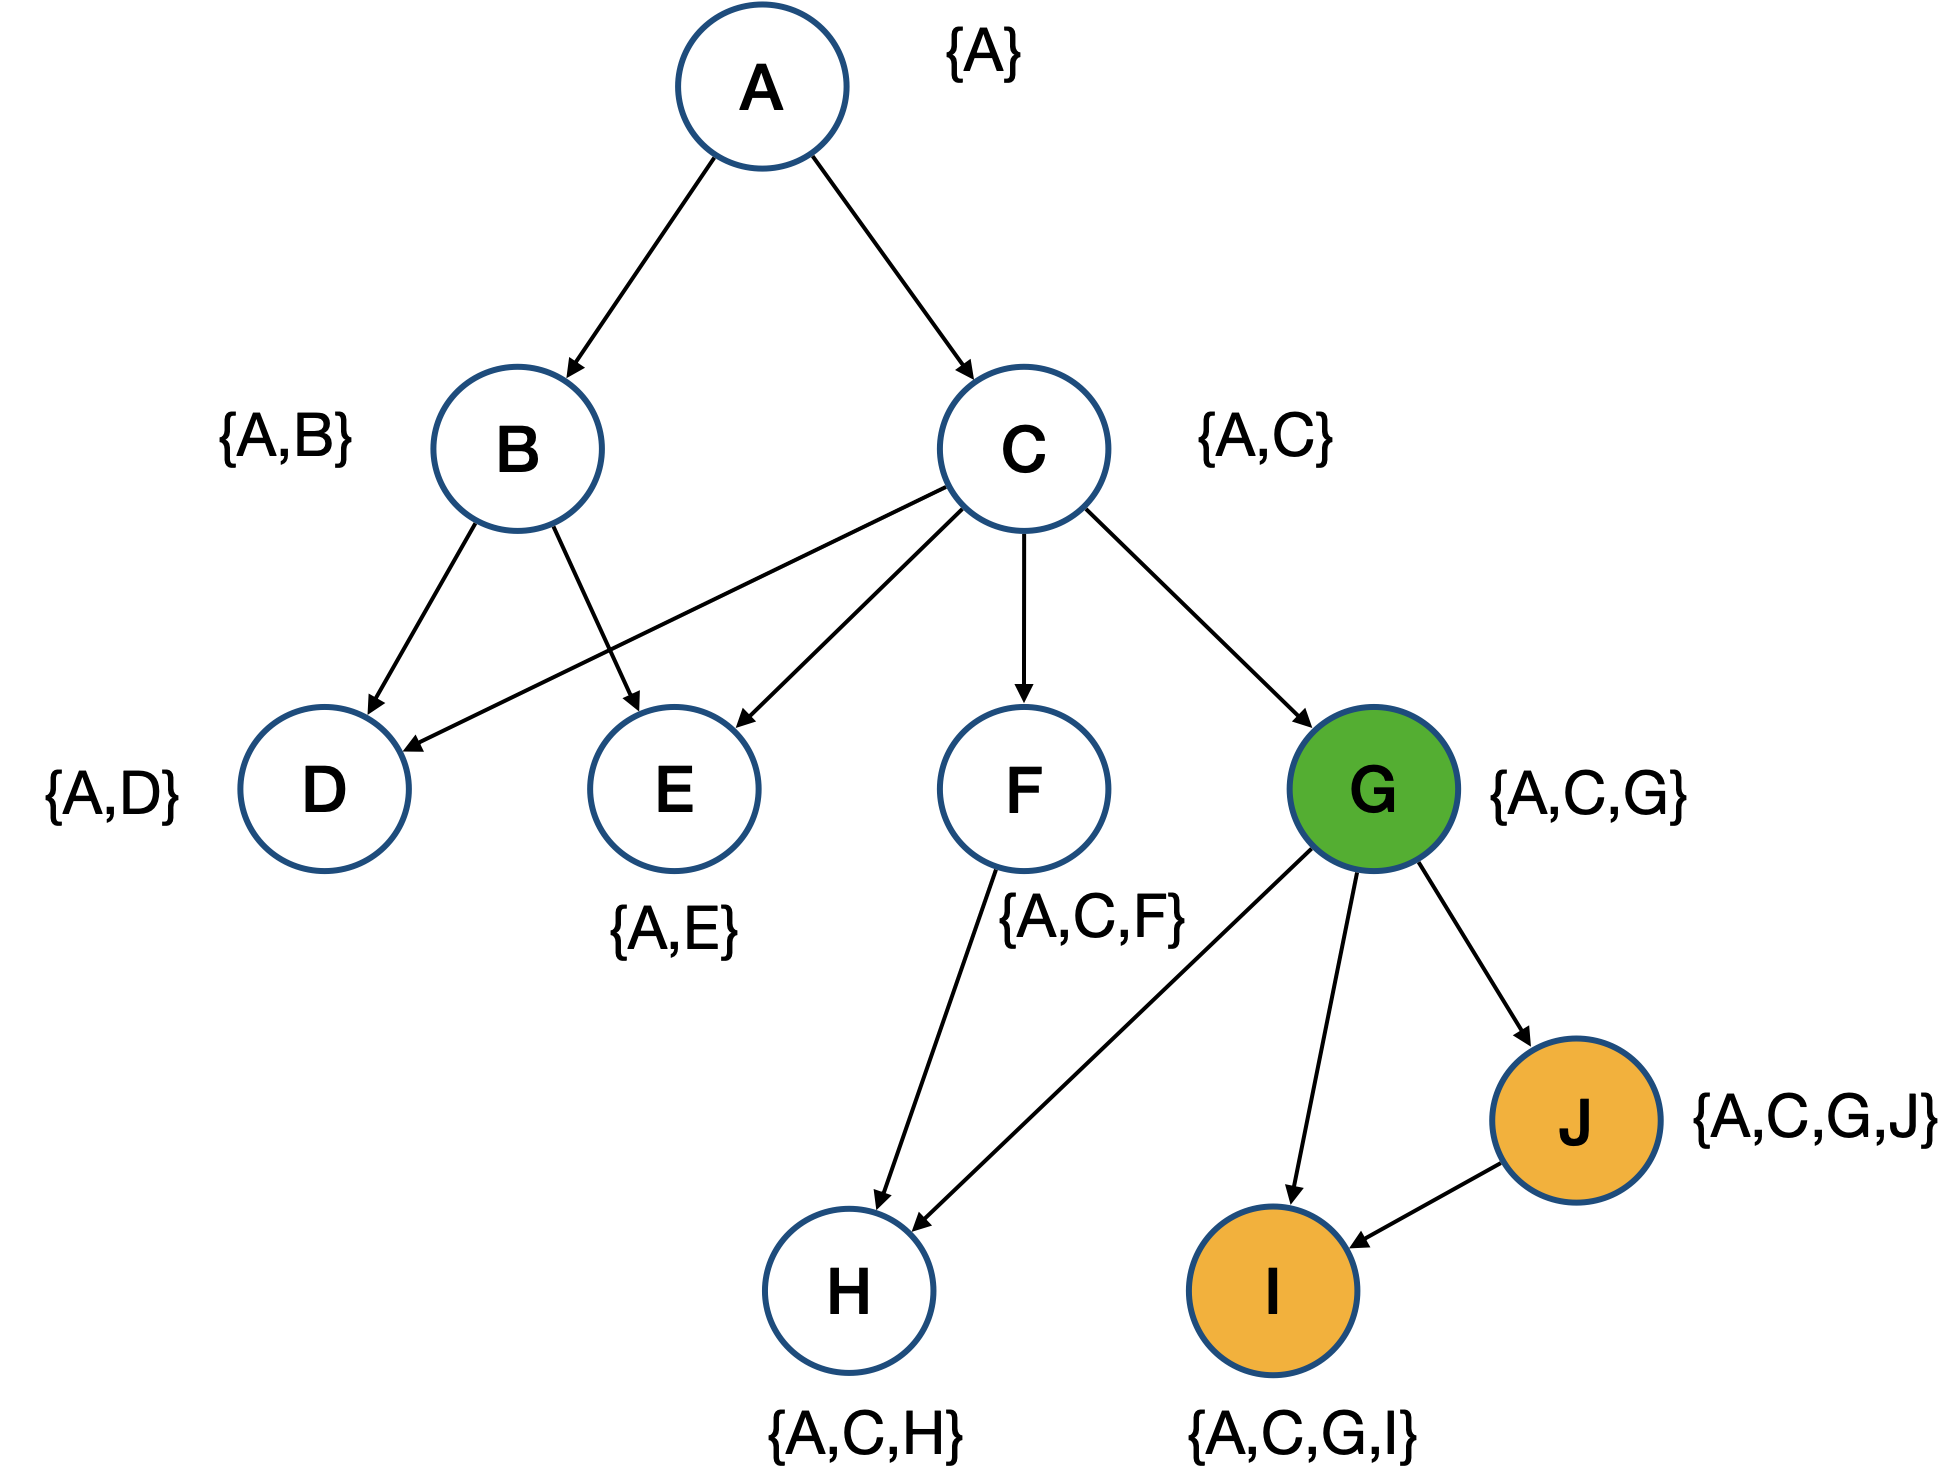
\includegraphics[width=0.6\textwidth]{figures/CALockExample.png}
	\caption{CALock labels on a hierarchy}
	\label{fig:calockexample}
\end{figure}

Then, the children of the vertex $v$ are explored via a breadth-first traversal over the graph. Using the labels of the parents, the label of the child is computed through Relation \ref{labellingRecursion}. For example, in Figure \ref{fig:calockexample}, the label of vertex $B$ is $\{A, B\}$ since it has only one parent. Vertex $E$ has two parents which have the labels $\{A, B\}$ and $\{A, C\}$ respectively. Their set intersection is $\{A\}$. Using Relation \ref{labellingRecursion}, the label of $E$ is $\{A, E\}$. The graph is explored and labelled until the recursion reaches a fix-point and terminates (line \ref{recursionCheck}). 

In acyclic graphs, this recursion reaches a fix-point when all the paths to the leaf vertices have been explored. By exploring the vertices in a depth-first manner, we ensure that the label of a vertex is computed only after the labels of all its parents have been computed so-as-to avoid recomputation as much as possible.


\begin{algorithm}[h]
	\caption{Labelling the graph}
	\begin{algorithmic}[1]
		\Procedure{AssignLabels}{v}
		\State $queue$.\Call{push}{v}
		\While{$queue$.\Call{hasNext}{ }}
		\State $v\gets queue.$\Call{Next}{ }
		\State \Call{BFLabelA}{v, queue}
		\EndWhile
		\EndProcedure
		\Statex

		\Procedure{BFLabelA}{v, queue}
		\State $C\gets$\Call{children}{v}
		\If{$parents(v) = \emptyset$ } \label{rootLabellingBegin}
		\State{$v.label\gets\{v\}$}
		\State $queue.$\Call{push}{ $C$ }
		\State return
		\EndIf\label{rootLabellingEnd}
		\State $P\gets$\Call{parents}{v}\label{labellingRelationImplBegin}
		\State $tempLabel\gets$\Call{Intersection}{P.$labels$}\label{intersectionStart}
		\State $tempLabel$.\Call{append}{v} \label{intersectionEnd}
		\If{$v.label \neq tempLabel$} \label{recursionCheck}
		\State $v.label\gets tempLabel$
		\State $queue.$\Call{push}{ $C$ }
		\EndIf \label{labellingRelationImplEnd}
		\EndProcedure
	\end{algorithmic}
	\label{labelAssignment}
\end{algorithm}


\subsubsection{Labelling a strongly connected component}
Strongly connected components are subgraphs that exhibit special properties in terms of connectivity of vertices. 
A strongly connected component is a maximal sub-graph of a directed graph where every vertex is reachable from every other. 
In Figure \ref{fig:stronglyConnectedComponent}, the cyan vertices form a strongly connected component.


\begin{figure}[H]
	\centering
	\captionsetup{justification=centering}
	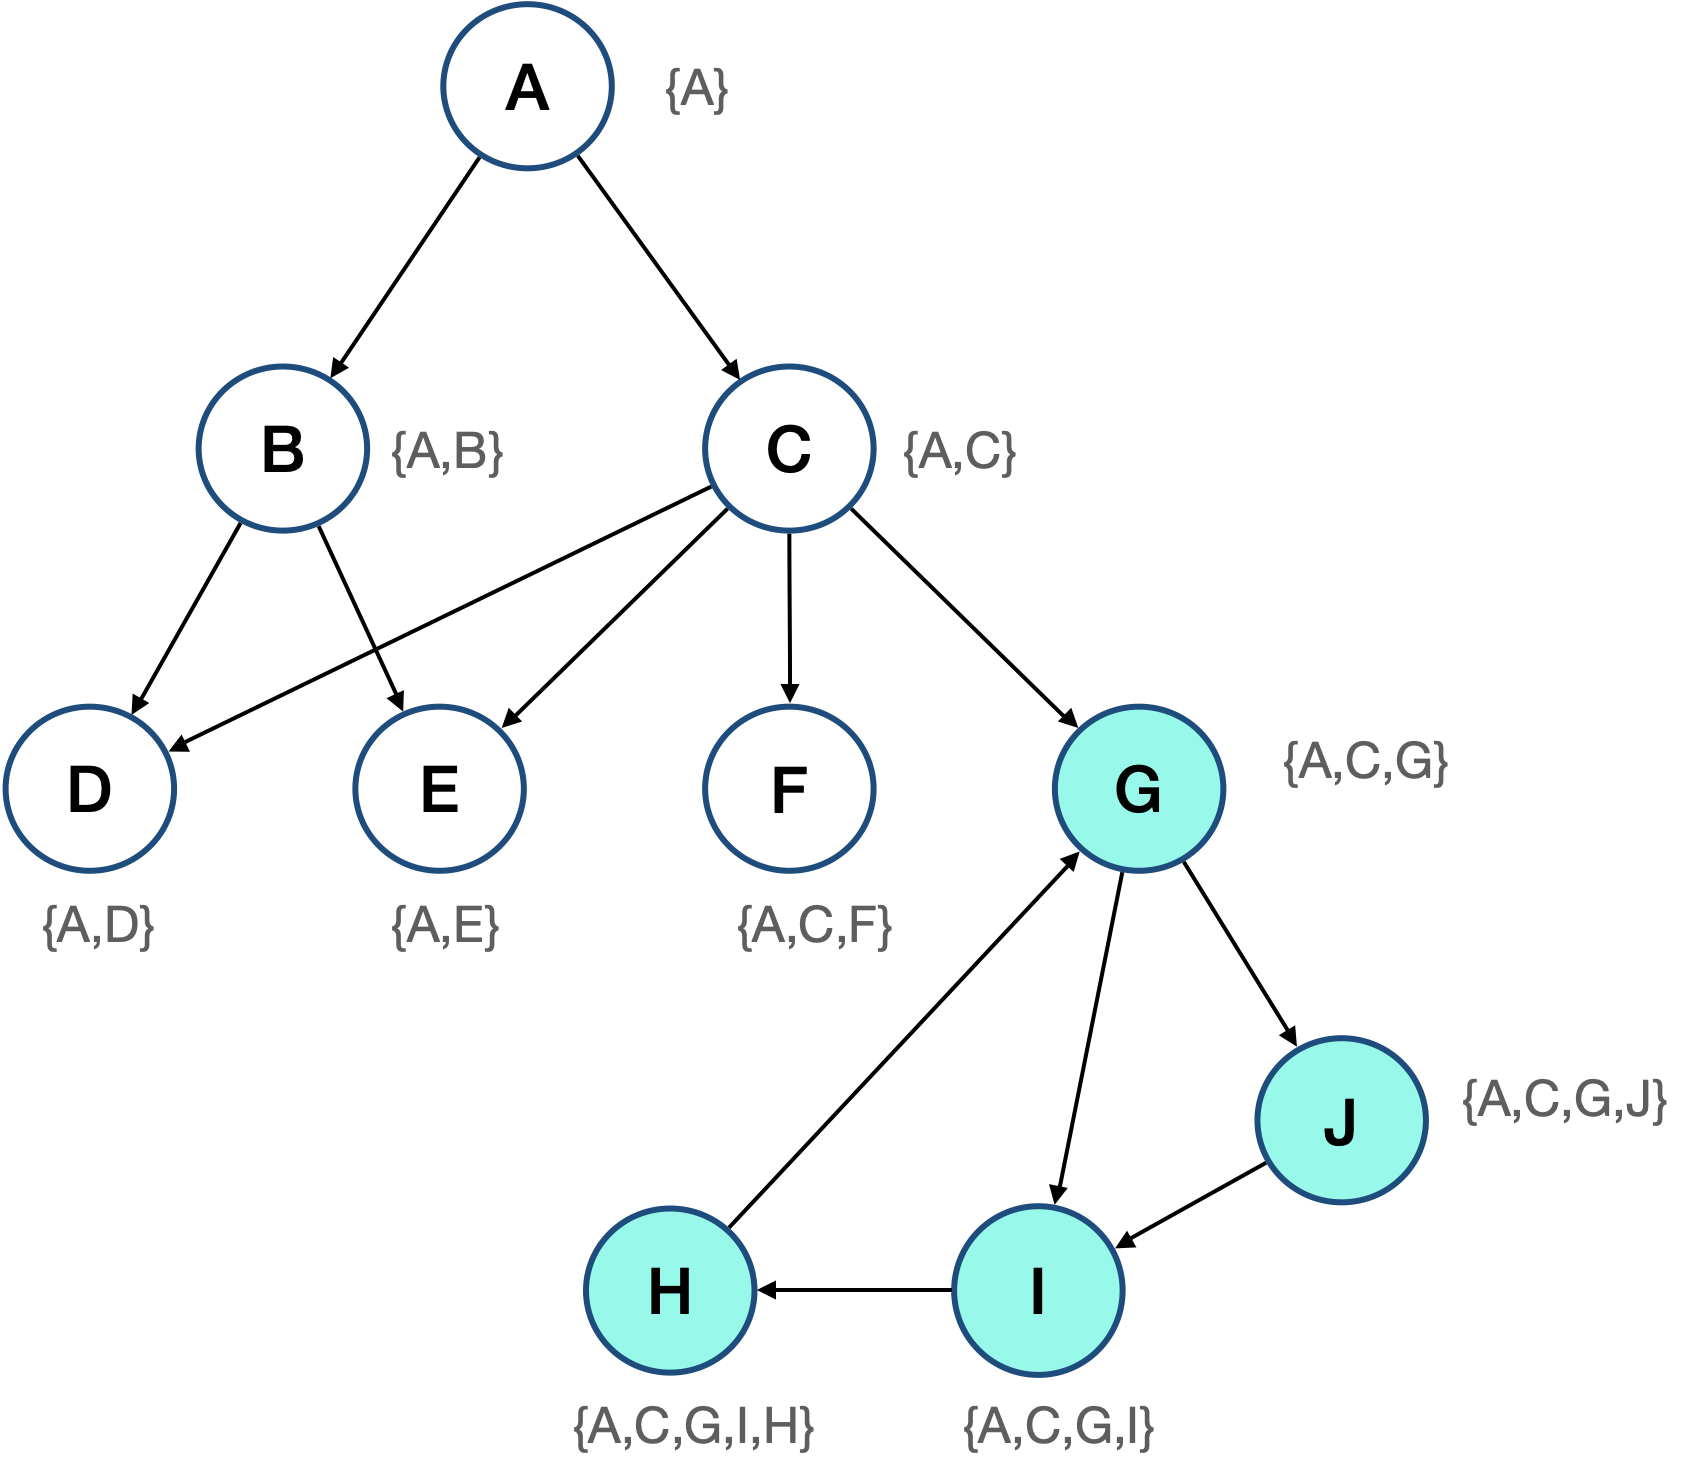
\includegraphics[width=0.6\textwidth]{figures/CALock_ConnectedComponent.png}
	\caption{CALock labels for a hierarchy containing strongly connected component (cyan)}
	\label{fig:stronglyConnectedComponent}
\end{figure}

Theorem \ref{proofOfDeepness} assumes that the graph does not contain strongly connected components. 
In real-life applications, maintaining this constraint is difficult. 
One approach to handling strongly connected components is to eliminate them by contracting the vertices in the component to a single vertex \cite{sharir1981strong, tarjan1972depth, cheriyan1996algorithms,walsh2006hub}. By doing so, we treat the strongly connected component as a single vertex in the graph. 
However, this approach alters the graph semantically which is not desirable in applications that store data in the vertices of the graph. By contracting the vertices, we lose the information stored in the vertices of the strongly connected component which is not acceptable. 
With the recursive relation \ref{labellingRecursion} we do not need to eliminate strongly connected components to label the vertices of a graph. 
% We, however, maintain that finding and eliminating strongly connected components is not required to identify lock grains with CALock when the labels are assigned using Relation \ref{labellingRecursion}. 
%This is because the label of a vertex in the connected component reaches a fix-point based on the topology of the graph.

% This is because when labelling with recursive Relation \ref{labellingRecursion}, the label of a vertex in the connected component reaches a fix-point based on the topology of the graph.


Assume that $N \subseteq V$ is a set of vertices of a graph that are strongly connected. Since every vertex in $N$ is reachable from every other vertex in $N$, the path set $\mathcal{P}_{(u,v)}$ for any pair of vertices $u, v\in N$ contains the same vertices and hence, every vertex in N has the same set of guarding ancestors. \inline|BFLabel| recurses over all vertices in $N$ until the paths labels of vertices in $N$ do not change any more (line \ref{recursionCheck}).
% Therefore, Relation \ref{labellingRecursion} is sufficient to label rooted directed graphs with strongly connected components.
For example, in Figure \ref{fig:stronglyConnectedComponent}, the vertices $G, H, I, J$ form a strongly connected component. 

\subsubsection{Relabelling a graph}

The topology of a graph can change due to \emph{structural modifications} which add or remove vertices and edges from a graph. 
Such modifications alter the topology of the graph and hence the paths that lead to a vertex from the root. 
When a structural modification occurs, the labels of the vertices need to be recomputed.

Unlike the other state-of-the-art techniques, which relabel the graph by performing the same post-order traversal from the left-most leaf, in CALock relabelling begins at the vertex affected by the structural modification via \lstinline|AssignLabel(v)| function. 
Unlike DomLock, MID and FlexiGran, CALock does not relabel the entire hierarchy when a structural modification occurs. 
It only relabels the affected vertices and their children. 
This is useful to not only parallelize structural modifications but also to reduce the overhead of relabelling the entire hierarchy.

In the same fashion as the initial labelling, the parents of $v$ are used to compute its label and recursively of its children. Relabelling terminates when it reaches a fix-point (line \ref{recursionCheck}).  

\begin{figure}[H]
	\centering
	\captionsetup{justification=centering}
	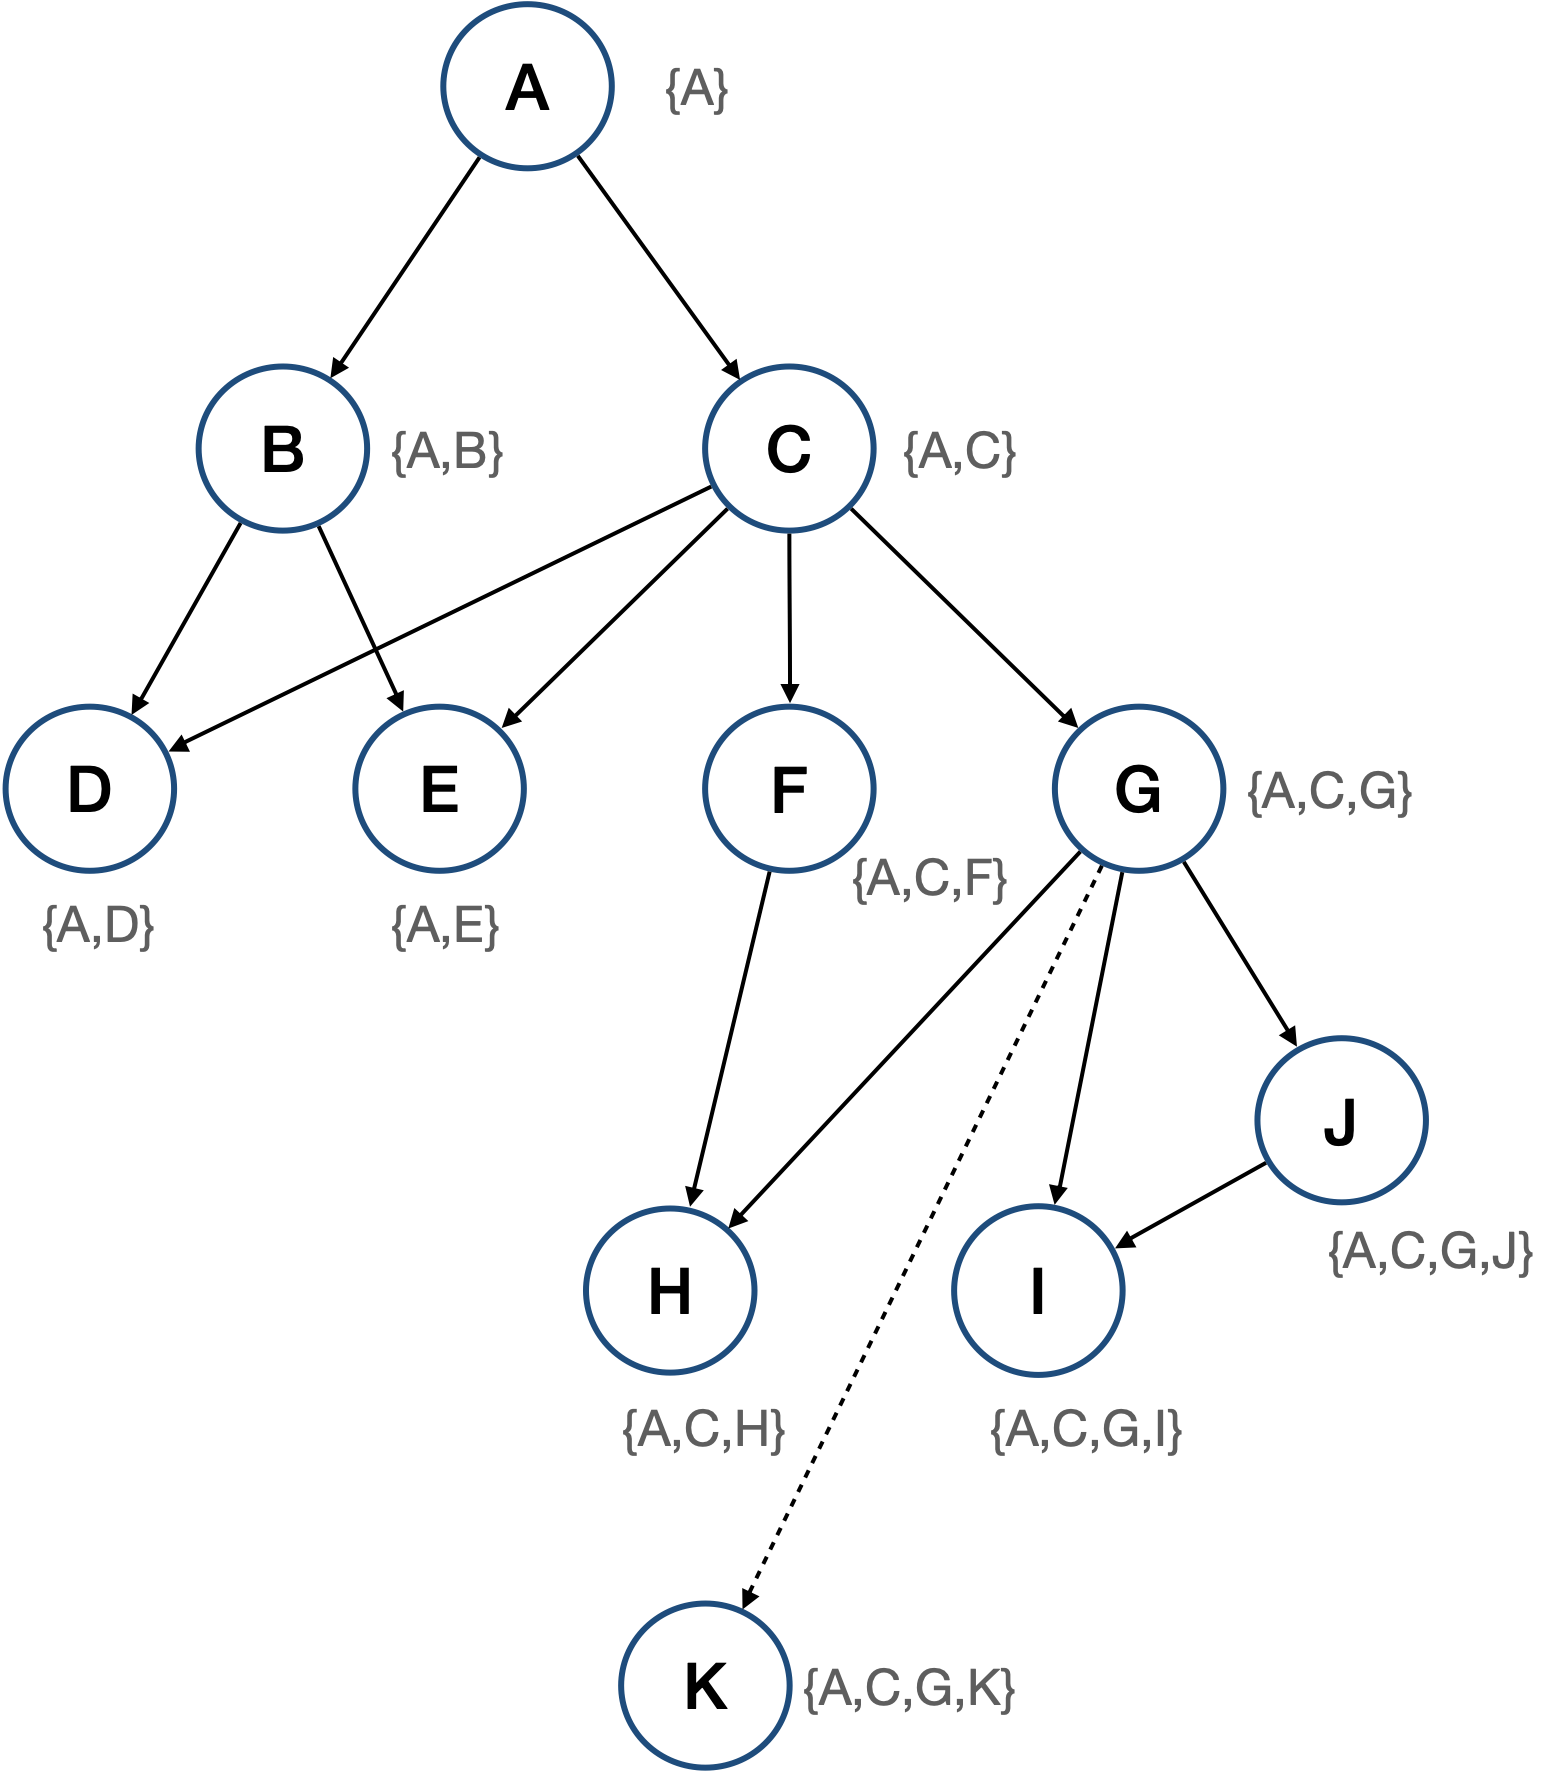
\includegraphics[width=0.6\textwidth]{figures/CALock_example_with_SM.png}
	\caption{CALock labels for a hierarchy with structural modifications}
	\label{fig:CAstructuralModification}
\end{figure}

Consider the example in Figure \ref{fig:CAstructuralModification}. Let us insert a new vertex $K$ as a child of G. The label of $K$ is the intersection of the labels of its parents i.e. $\{A,C,G,K\}$. Since $K$ is a leaf vertex, the recursion terminates. 
No other vertex in the hierarchy is relabelled. 
This allows CALock to efficiently handle structural modifications in the hierarchy by eliminating the need of a mutex for relabelling the entire hierarchy and by parallelizing the relabelling process. 



